\documentclass[border=2pt]{standalone}
\usepackage{amssymb,amsmath}
\usepackage{tikz-cd}
\usepackage{physics}
\usetikzlibrary{arrows}

\usepackage{tikz}
\let\OX\bigotimes
\newcommand{\OP}{\displaystyle\bigoplus}
\let\ox\otimes
\let\op\oplus
\let\isom\cong
\let\vf\varphi
\begin{document}



\tikzset{every picture/.style={line width=0.75pt}} %set default line width to 0.75pt        

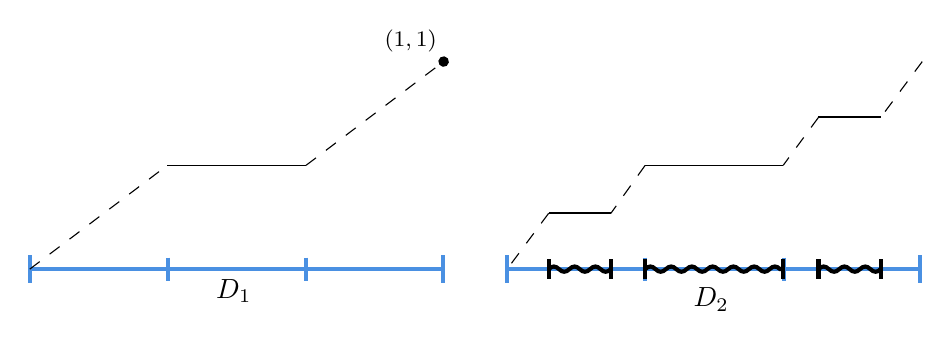
\begin{tikzpicture}[x=0.75pt,y=0.75pt,yscale=-1,xscale=1]
%uncomment if require: \path (0,300); %set diagram left start at 0, and has height of 300

%Straight Lines [id:da5805086794975216] 
\draw  [dash pattern={on 4.5pt off 4.5pt}]  (290,173.1) -- (270,200) ;
%Straight Lines [id:da5059750287178231] 
\draw [color={rgb, 255:red, 74; green, 144; blue, 226 }  ,draw opacity=1 ][line width=1.5]    (40,200) -- (239,200) (106.6,194.5) -- (106.6,205.5)(173.2,194.5) -- (173.2,205.5) ;
\draw [shift={(239,200)}, rotate = 180] [color={rgb, 255:red, 74; green, 144; blue, 226 }  ,draw opacity=1 ][line width=1.5]    (0,6.71) -- (0,-6.71)   ;
\draw [shift={(40,200)}, rotate = 180] [color={rgb, 255:red, 74; green, 144; blue, 226 }  ,draw opacity=1 ][line width=1.5]    (0,6.71) -- (0,-6.71)   ;
%Straight Lines [id:da7785005596126242] 
\draw [color={rgb, 255:red, 74; green, 144; blue, 226 }  ,draw opacity=1 ][line width=1.5]    (270,200) -- (469,200) (336.6,194.5) -- (336.6,205.5)(403.2,194.5) -- (403.2,205.5) ;
\draw [shift={(469,200)}, rotate = 180] [color={rgb, 255:red, 74; green, 144; blue, 226 }  ,draw opacity=1 ][line width=1.5]    (0,6.71) -- (0,-6.71)   ;
\draw [shift={(270,200)}, rotate = 180] [color={rgb, 255:red, 74; green, 144; blue, 226 }  ,draw opacity=1 ][line width=1.5]    (0,6.71) -- (0,-6.71)   ;
%Straight Lines [id:da9044418526344229] 
\draw [line width=1.5]    (290,200) .. controls (291.67,198.33) and (293.33,198.33) .. (295,200) .. controls (296.67,201.67) and (298.33,201.67) .. (300,200) .. controls (301.67,198.33) and (303.33,198.33) .. (305,200) .. controls (306.67,201.67) and (308.33,201.67) .. (310,200) .. controls (311.67,198.33) and (313.33,198.33) .. (315,200) .. controls (316.67,201.67) and (318.33,201.67) .. (320,200) -- (320,200) ;
\draw [shift={(320,200)}, rotate = 180] [color={rgb, 255:red, 0; green, 0; blue, 0 }  ][line width=1.5]    (0,4.7) -- (0,-4.7)   ;
\draw [shift={(290,200)}, rotate = 180] [color={rgb, 255:red, 0; green, 0; blue, 0 }  ][line width=1.5]    (0,4.7) -- (0,-4.7)   ;
%Straight Lines [id:da017574628734651654] 
\draw [line width=1.5]    (420,200) .. controls (421.67,198.33) and (423.33,198.33) .. (425,200) .. controls (426.67,201.67) and (428.33,201.67) .. (430,200) .. controls (431.67,198.33) and (433.33,198.33) .. (435,200) .. controls (436.67,201.67) and (438.33,201.67) .. (440,200) .. controls (441.67,198.33) and (443.33,198.33) .. (445,200) .. controls (446.67,201.67) and (448.33,201.67) .. (450,200) -- (450,200) ;
\draw [shift={(450,200)}, rotate = 180] [color={rgb, 255:red, 0; green, 0; blue, 0 }  ][line width=1.5]    (0,4.7) -- (0,-4.7)   ;
\draw [shift={(420,200)}, rotate = 180] [color={rgb, 255:red, 0; green, 0; blue, 0 }  ][line width=1.5]    (0,4.7) -- (0,-4.7)   ;
%Straight Lines [id:da28869711544283705] 
\draw [line width=1.5]    (336.5,200) .. controls (338.17,198.33) and (339.83,198.33) .. (341.5,200) .. controls (343.17,201.67) and (344.83,201.67) .. (346.5,200) .. controls (348.17,198.33) and (349.83,198.33) .. (351.5,200) .. controls (353.17,201.67) and (354.83,201.67) .. (356.5,200) .. controls (358.17,198.33) and (359.83,198.33) .. (361.5,200) .. controls (363.17,201.67) and (364.83,201.67) .. (366.5,200) .. controls (368.17,198.33) and (369.83,198.33) .. (371.5,200) .. controls (373.17,201.67) and (374.83,201.67) .. (376.5,200) .. controls (378.17,198.33) and (379.83,198.33) .. (381.5,200) .. controls (383.17,201.67) and (384.83,201.67) .. (386.5,200) .. controls (388.17,198.33) and (389.83,198.33) .. (391.5,200) .. controls (393.17,201.67) and (394.83,201.67) .. (396.5,200) .. controls (398.17,198.33) and (399.83,198.33) .. (401.5,200) -- (403,200) -- (403,200) ;
\draw [shift={(403,200)}, rotate = 180] [color={rgb, 255:red, 0; green, 0; blue, 0 }  ][line width=1.5]    (0,4.7) -- (0,-4.7)   ;
\draw [shift={(336.5,200)}, rotate = 180] [color={rgb, 255:red, 0; green, 0; blue, 0 }  ][line width=1.5]    (0,4.7) -- (0,-4.7)   ;
%Straight Lines [id:da6802426497933824] 
\draw    (106.3,150) -- (173.1,150) ;
%Straight Lines [id:da5013372545613453] 
\draw  [dash pattern={on 4.5pt off 4.5pt}]  (40,200) -- (106.3,150) ;
%Straight Lines [id:da7641293449177631] 
\draw  [dash pattern={on 4.5pt off 4.5pt}]  (173.1,150) -- (239.4,100) ;
\draw [shift={(239.4,100)}, rotate = 322.98] [color={rgb, 255:red, 0; green, 0; blue, 0 }  ][fill={rgb, 255:red, 0; green, 0; blue, 0 }  ][line width=0.75]      (0, 0) circle [x radius= 2.01, y radius= 2.01]   ;
%Straight Lines [id:da30242118947256347] 
\draw    (336.5,150) -- (403,150) ;
%Straight Lines [id:da4984076806413744] 
\draw [line width=0.75]    (290,173.1) -- (320,173.1) ;
%Straight Lines [id:da10825727518306372] 
\draw [line width=0.75]    (420,126.9) -- (450,126.9) ;
%Straight Lines [id:da6978281220865536] 
\draw  [dash pattern={on 4.5pt off 4.5pt}]  (336.5,150) -- (320,173.1) ;
%Straight Lines [id:da7183182118630689] 
\draw  [dash pattern={on 4.5pt off 4.5pt}]  (420,126.9) -- (403,150) ;
%Straight Lines [id:da6650389751609507] 
\draw  [dash pattern={on 4.5pt off 4.5pt}]  (470,100) -- (450,126.9) ;

% Text Node
\draw (237.4,96.6) node [anchor=south east] [inner sep=0.75pt]  [font=\footnotesize]  {$( 1,1)$};
% Text Node
\draw (128.57,203.83) node [anchor=north west][inner sep=0.75pt]    {$D_{1}$};
% Text Node
\draw (358.57,207.83) node [anchor=north west][inner sep=0.75pt]    {$D_{2}$};


\end{tikzpicture}


\end{document}